\documentclass[oneside]{htwg-report}

% Use german umlaute
\usepackage{german,ngerman}
\usepackage[T1]{fontenc}
\usepackage[utf8]{inputenc}
\usepackage[ngerman]{babel}
\usepackage[autostyle=true,german=quotes]{csquotes}

%\usepackage[table]{xcolor}\usepackage{float}
%\usepackage{xcolor,colortbl}

\addbibresource{./bib/report.bib}

\begin{document}

\pagenumbering{gobble}

%% 'reporttype' add background elements to the cover / front page
%% possible values are:
%% bachelor	--> B S C
%% master	--> M S C
%% other		--> none
\reporttype{master}

\reporttypetext{Teamproject (Master 3. semester)}

\newcommand{\verfasserA}{Simon Christofzik}
\newcommand{\verfasserB}{Paul Sutter}
\newcommand{\verfasserC}{Till Reitlinger}
\newcommand{\thema}{DeepRain: Rain forecast with neural networks and the visualization of these in an App}
\newcommand{\hoschschule}{HTWG Konstanz - University of Applied Sciences}
\newcommand{\institut}{HTWG Konstanz - Institute for Optical Systems}
\newcommand{\prueferA}{Prof. Dr. Oliver Dürr}


\title[Teamprojektthema]{\thema}

\doclocation{Konstanz}
\docdate{10. September 2020}

\makecover[]

\chapter*{Extended Abstract}

\begin{center}
	\begingroup
	\renewcommand*{\arraystretch}{1}
	\rowcolors{2}{white}{white}
	{\makeatletter	
		\begin{tabular}{p{3.2cm}p{9.6cm}}
			Topic: & \thema \\
			& \\
			Team members: & \verfasserA, \verfasserB, \verfasserC \\
			& \\
			Advisor: & \hoschschule \newline \institut \newline \prueferA \\
			& \\
		\end{tabular}
		
		\makeatother}
	\endgroup
\end{center}

\bigskip

In this Paper we try to predict precipitation for a range of 35 minutes in an area around Constance.
Therefore we are using machine learning techniques and train a UNet on radar data images. 
Here we present the result of precipitation prediction as well with regression as with classification. 
Both approaches provide good results. Source code and full length documentation in german can be found at GitHub: \url{https://github.com/thgnaedi/DeepRain}.


\printbibliography[title={References}, heading=subbibliography]


\twocolumn
\section*{Introduction}

\begin{sloppypar}
\tolerance 9999
Even today, rain forecasts are still very computationally complex and relatively inaccurate. 
Therefore, it may make sense to make such predictions with the help of neural networks. 
These do not require as much computing power and can recognize a pattern in the often chaotic data even without complex physical models.
\end{sloppypar}

\section*{Data}\label{data}
Images must be generated from the binary radar data provided by the German Weather Service (DWD) in five-minute resolution.
To convert the radar data into an image, each radar data point must be transformed into a pixel color value.
In order to achieve a suitable transformation, the radar data of June 2016 were inspected exemplarily (figure \ref{fig:Radardatapoints_of_June_2016}). 

\begin{figure}[ht]
    \centering
    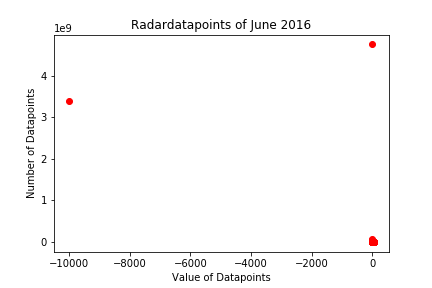
\includegraphics[width=1\linewidth,angle=0]{../abb/Radardatapoints_of_June_2016.png}
    \caption[Datenaufbereitung]{Frequency distribution of rain data}
    \label{fig:Radardatapoints_of_June_2016}
\end{figure}

All occurring values and their frequency are plotted. 
Two outliers stand out in figure \ref{fig:Radardatapoints_of_June_2016}, which occur much more frequently than the other values. 
The value -9999 indicates that no data is available and the second outlier is at 0, which stands for \"no rain\". 
In Figure \ref{fig:Radardatapoints_of_June_2016_larger0_99percentile} the two outliers are filtered, because the relevant information is contained in the remaining data points.
In addition, the 99\% percentile illustrates the frequency distribution. 

\begin{figure}[ht]
    \centering
    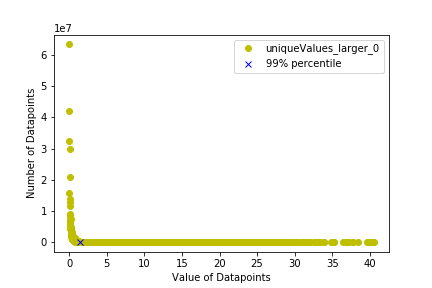
\includegraphics[width=1\linewidth,angle=0]{../abb/Radardatapoints_of_June_2016_larger0_99percentile.png}
    \caption[Datenaufbereitung]{Frequency distribution of rain data with 99\% percentile}
    \label{fig:Radardatapoints_of_June_2016_larger0_99percentile}
\end{figure}

The 99\% percentile contains 138 different values, each of which is assigned a color value.
The remaining data is transformed linearly to the remaining range of values.
This results in rounding and maximum value errors. These errors are bearable, because it is more important to map all data points.
Furthermore the resolution of the different rainfall intensities is still higher than the human perception.
Reconstructing the radar data from the PNG data results in the plot shown in figure \ref{fig:Radardatapoints_of_June_2016_RecoveredData}.

\begin{figure}[ht]
    \centering
    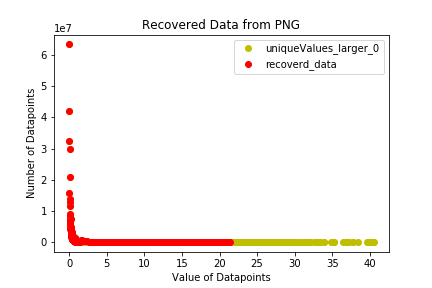
\includegraphics[width=1\linewidth,angle=0]{../abb/Radardatapoints_of_June_2016_RecoveredData.png}
    \caption[Datenaufbereitung]{Comparison between output distribution and distribution from recovered data}
    \label{fig:Radardatapoints_of_June_2016_RecoveredData}
\end{figure}






\section*{Data Validation}\label{data validation}

To validate the quality of the data as well as the correct position of the constant pixel, the radar data were compared with the weather station in Konstanz.
The radar data of one week from all over Germany were correlated with the weather station.
The correlation coefficient reached its maximum around Konstanz.
There are deviations from radar data to rainfall compensation, especially with small rainfall values, but these are caused by inaccuracies of the weather station itself (figure \ref{fig:radar_station_daten_vergleich_June}).
The correlation is significant, the position of Konstanz could be validated and the data quality is suitable for a rain forecast.

\begin{figure}[ht]
    \centering
    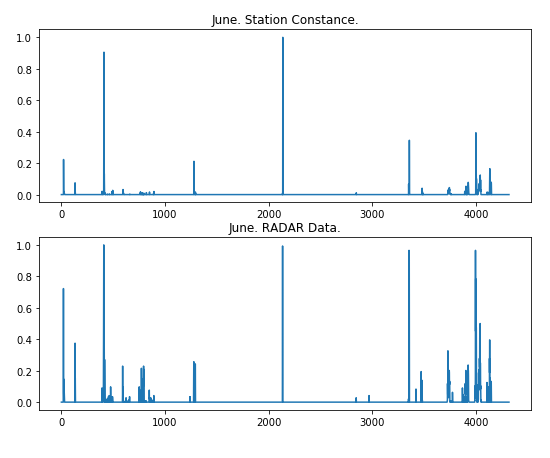
\includegraphics[width=1\linewidth,angle=0]{../abb/radar_station_daten_vergleich_June.png}
    \caption[Datenaufbereitung]{Comparison between Radar and Weatherstation in June 2016}
    \label{fig:radar_station_daten_vergleich_June}
\end{figure}

\begin{figure}[ht]
\centering
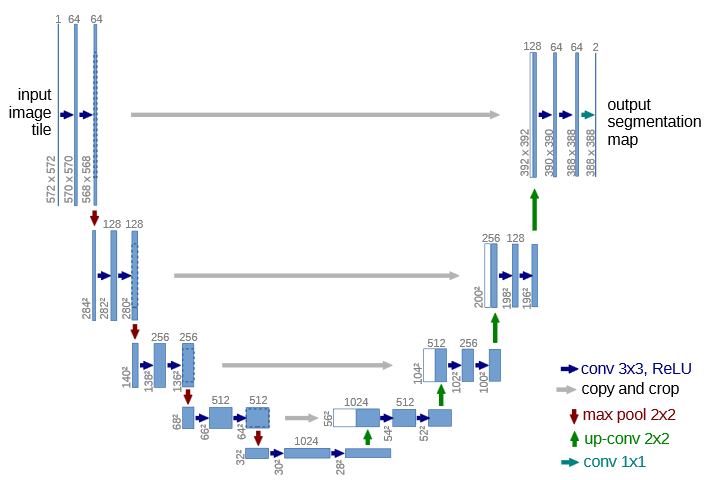
\includegraphics[width=0.8\linewidth]{../abb/UNet_Biomedical}
\caption{The image is taken from the university of Freiburg~\cite{ronneberger2015u}}
\end{figure}

\begin{sloppypar}
\tolerance 9999
\noindent
\end{sloppypar}

\section*{DeepRain Application}

\begin{figure}[ht]
    \centering
    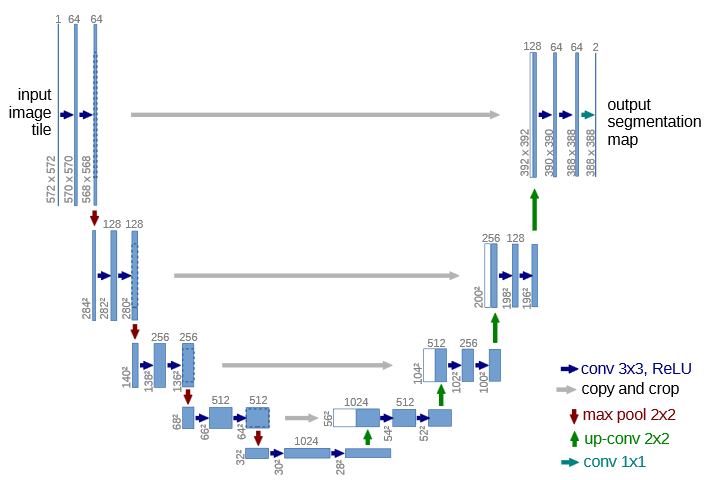
\includegraphics[width=0.8\linewidth]{../abb/UNet_Biomedical}
    \caption{The image is taken from the university of Freiburg~\cite{ronneberger2015u}}
\end{figure}


\begin{figure}[ht]
    \centering
    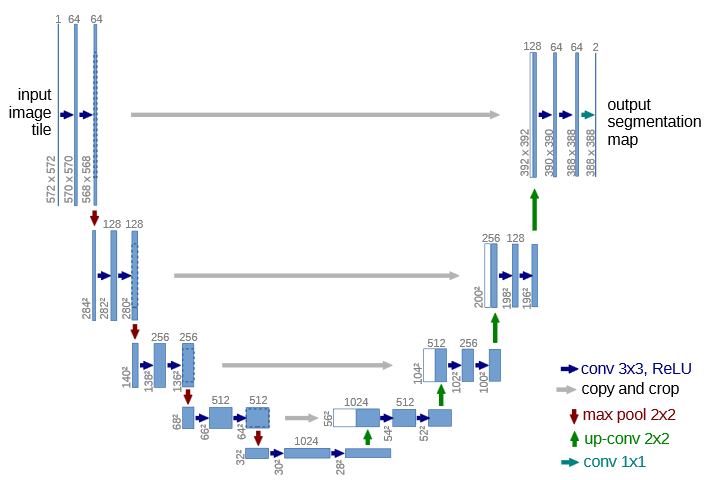
\includegraphics[width=0.8\linewidth]{../abb/UNet_Biomedical}
    \caption{The image is taken from the university of Freiburg~\cite{ronneberger2015u}}
\end{figure}



\section*{Pipeline}

\begin{figure}[ht]
    \centering
    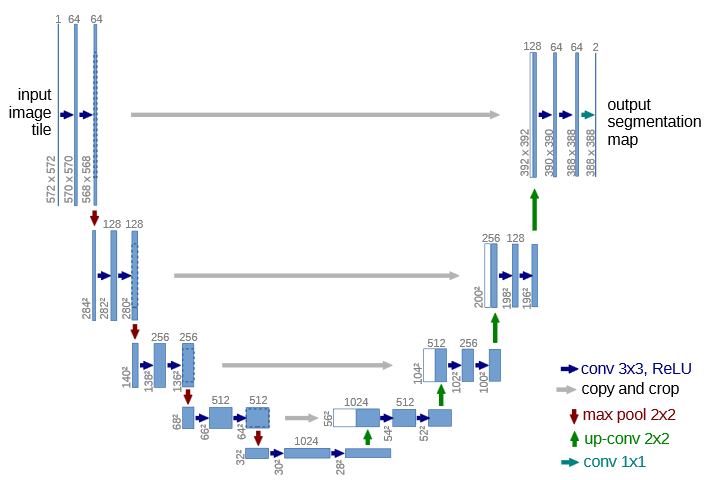
\includegraphics[width=0.8\linewidth]{../abb/UNet_Biomedical}
    \caption{The image is taken from the university of Freiburg~\cite{ronneberger2015u}}
\end{figure}



\begin{figure}[ht]
    \centering
    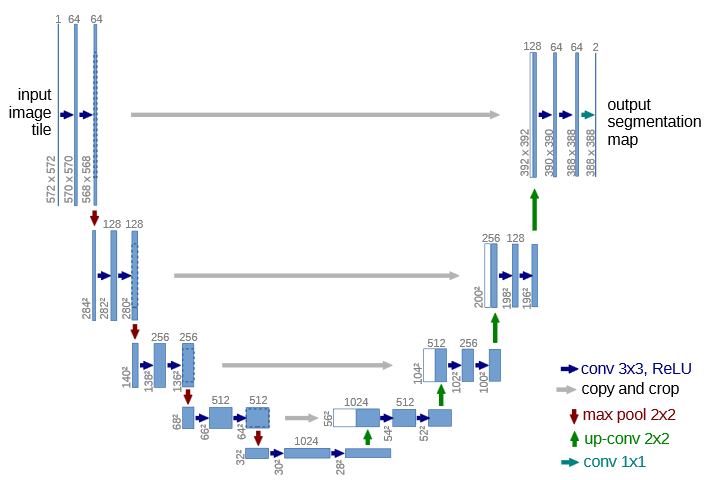
\includegraphics[width=0.8\linewidth]{../abb/UNet_Biomedical}
    \caption{The image is taken from the university of Freiburg~\cite{ronneberger2015u}}
\end{figure}

\section*{Conclusion and Future Work}


\end{document}

